% primary source: [Análise sintática usando `bison`](https://docs.google.com/presentation/d/1laBDtX7fnyZmFdUaTAizxFqYeuT55bg3rTAh_SdAHXo/edit?usp=sharing)

\title{Análise sintática usando {\tt yacc}}
\section{Análise sintática usando {\tt yacc} (bison)}

\frame{\maketitle}

\frame{\tableofcontents}

\subsection{Análise sintática}

\begin{frame}{Análise ascendente}{{\em Bottom-up parsing}}
  LALR ({\it Lookahead Left-right Rightmost derivation\/})

  \begin{columns}
     \begin{column}{.5\textwidth}
      \begin{block}{Gramática}
        \begin{tabbing}
          E \= $\rightarrow$ \= E + T \= | T \\
          T \> $\rightarrow$ \> T * F \> | F\\
          F \> $\rightarrow$ \> ( E ) \> | {\bf digit}\\
        \end{tabbing}
        \{+, *, (, ), {\bf digit}\} $\in$ terminais;\\
        \{E, F, T\} $\in$ não-terminais;\\
        \{{\bf digit}\} $\in$ símbolo de início ({\it rightmost\/});\\
        $\rightarrow$: regras de produção.
      \end{block}
    \end{column}
    \pause
    \begin{column}{.5\textwidth}
      \begin{block}{Árvore sintática ({\it parser tree\/})}
        {\bf 2} * {\bf 3}\\ 
        \small
      \begin{tikzpicture}
        \node {E}
          child {node {T}
            child {node {T}
              child {node {F}
                child {node {\bf 2}}
              }
            }
            child {node {\bf *}}
            child {node {F}
              child {node {\bf 3}}
            }
          };
      \end{tikzpicture}
    \end{block}
    \end{column}
  \end{columns}
\end{frame}

\subsection{yacc}

\begin{frame}{yacc}{bison}
  \begin{description}
  \item[yacc]  ``Yet Another Compiler Compiler''
    \begin{itemize}
    \item Gerador de analisador sintático ({\it parser\/});
    \item \alert{\tt bison} - substituto de código aberto.
      \begin{itemize}
      \item C++, thread-safe;
      \item Converte gramática livre de contexto anotada usando
        LALR\footnote{{\it Lookahead Left-right (bottom-up) with
          Rightmost derivation\/}}.
      \end{itemize}
    \end{itemize}
  \end{description}
\end{frame}

\frame{\frametitle{Fluxo de compilação}\center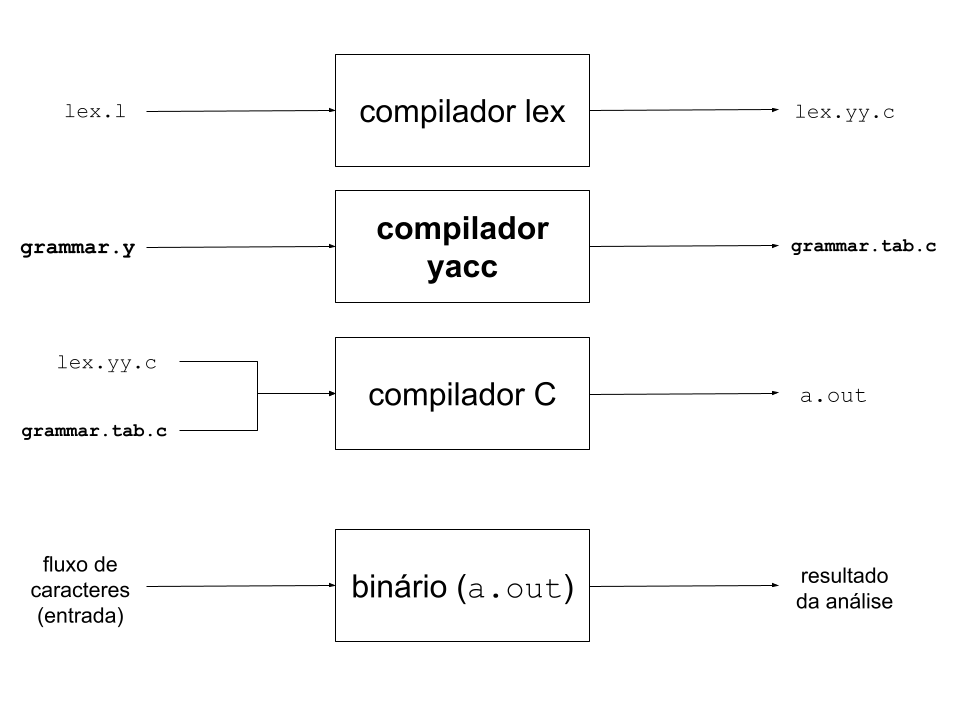
\includegraphics[scale=.35]{yacc-compilador.png}}

\begin{frame}[fragile]{Seções do arquivo}
\begin{lstlisting}
declarações

%%

regras gramaticais e ações

%%

código em C

\end{lstlisting}
\end{frame}

\subsection{Exemplo de especificação de gramática}

\frame{\tableofcontents[currentsubsection]}

\begin{frame}[fragile]{Exemplo}{Expecificação de gramática usando yacc}

  {\hfil\color{gray} Calculadora de mesa simples}\bigskip

  \begin{columns}
    \begin{column}{.35\textwidth}
      \begin{block}{Gramática}
        \begin{tabbing}
          E \= $\rightarrow$ \= E + T \= | T \\
          T \> $\rightarrow$ \> T * F \> | F\\
          F \> $\rightarrow$ \> ( E ) \> | {\bf digit}\\
        \end{tabbing}
      \end{block}
    \end{column}
    \scriptsize
    \pause
    \begin{column}{.65\textwidth}
      \begin{lstlisting}
%union {
        int d;
}
%token <d> DIGIT
%type  <d> expr term factor

%%
line   : expr '\n'         { printf("%d\n", $1); }
       ;
expr   : expr '+' term     { $$ = $1 + $3; }
       | term
       ;
term   : term '*' factor   { $$ = $1 * $3; }
       | factor
       ;
factor : '(' expr ')'      { $$ = $2; }
       | DIGIT
       ;
%%
      \end{lstlisting}
    \end{column}
  \end{columns}
\end{frame}

\note{O próximo slide é a explicação do bison executando em modo debug
  para a saída da calculadora de mesa simples.}
\begin{frame}{{\tt bison} LALR: exemplo}{reduções e deslocamentos}
\centering\small
  \begin{tikzpicture}[>=latex]
    \node (two) {{\tt 2}};
    \node (plus) [right of=two] {{\tt +}};
    \node (one) [right of=plus] {{\tt 1}};
    \node (times) [right of=one] {{\tt *}};
    \node (three) [right of=times] {{\tt 3}};
    \node (nl) [right of=three] {{\tt '$\backslash$n'}};
    \only<-5>{
      \node (pointer) [below of=two] {};
      \draw[->] (pointer) -- (two);
    }
    \only<6>{
      \node (pointer) [below of=plus] {};
      \draw[->] (pointer) -- (plus);
    }
    \only<7-9>{
      \node (pointer) [below of=one] {};
      \draw[->] (pointer) -- (one);
    }
    \only<10>{
      \node (pointer) [below of=times] {};
      \draw[->] (pointer) -- (times);
    }
    \only<11-12>{
      \node (pointer) [below of=three] {};
      \draw[->] (pointer) -- (three);
    }
    \only<13-15>{
      \node (pointer) [below of=nl] {};
      \draw[->] (pointer) -- (nl);
    }
    \only<13>{
      \node (pointer) [below of=one] {$3$};
    }
    \only<14->{
      \node (pointer) [below of=one] {$5$};
    }
  \end{tikzpicture}\bigskip

  \scriptsize
  \begin{tabular}[h]{r|l|c|l}
    \toprule
    & \hfil pilha & entrada &\hfil ação \\
    \midrule
    (1) &   &\hfill {\bf digit} + {\bf digit} * {\bf digit}\$& desloca \\
    \only<2->{
    (2) &  {\bf digit} &\hfill + {\bf digit} * {\bf digit}\$ & reduz: $F\rightarrow$ {\bf digit} \\
    }
    \only<3->{
    (3) & $F$ &\hfill + {\bf digit} * {\bf digit}\$ & reduz: $F\rightarrow T$ \\
    }
    \only<4->{
    (4) & $T$ &\hfill + {\bf digit} * {\bf digit}\$ & reduz: $T\rightarrow E$ \\
    }
    \only<5->{
    (5) & $E$ &\hfill + {\bf digit} * {\bf digit}\$ & desloca \\
    }
    \only<6->{
    (6) & $E+$ &\hfill {\bf digit} * {\bf digit}\$ & desloca \\
    }
    \only<7->{
    (7) & $E+$ {\bf digit} &\hfill  * {\bf digit}\$ & reduz: $F\rightarrow$ {\bf digit} \\
    }
    \note{aqui lookahead no * para decidir a próxima ação}
    \only<8->{
    (8) &  $E+F$ &\hfill  * {\bf digit}\$ & reduz: $T\rightarrow F$ \\
    }
    \only<9->{
    (9) &  $E+T$ &\hfill  * {\bf digit}\$ & desloca \\}
    \note{aqui lookahead no digit para decidir a próxima ação}
    \only<10->{
    (10) & $E+T*$ &\hfill {\bf digit}\$ & desloca \\
    }
    \only<11->{
    (11) & $E+T*${\bf digit} &\hfill \$ & reduz: $F\rightarrow$ {\bf digit} \\
    }
    \only<12->{
    (12) & $E+T*F$ &\hfill \$ & reduz: $T\rightarrow T*F$ \\
    }
    \note{aqui lookahead no newline para decidir a próxima ação}
    \only<13->{
    (13) & $E+T$ &\hfill \$ & reduz: $E\rightarrow E+T$ \\
    }
    \only<14->{
    (14) & $E$ &\hfill \$ & desloca {\tt '$\backslash$n'} \\
    }
    \only<15->{
    (15) & $E${\tt '$\backslash$n'} &\hfill \$ & reduz: $L\rightarrow E${\tt '$\backslash$n'} \\
    }
    \only<16>{
    (16) & $L$ &\hfill \$ & aceita \\
    }


    & & & \\
   \bottomrule
  \end{tabular}
\end{frame}

\begin{frame}[fragile]{{\tt flex} + {\tt bison}}{lex + yacc}
  {\hfil\color{gray} Calculadora de mesa simples}\bigskip

  \begin{columns}
    \begin{column}{.45\textwidth}\scriptsize
\begin{lstlisting}
%%
[0-9]     { yylval.d = atoi(yytext);
            return DIGIT;
          }
[*+()\n]  { return yytext[0]; }
[ \t]     { ; /* ignore */ }
.         {
            yyerror("erro");
          }
%%
\end{lstlisting}
\end{column}\scriptsize
\begin{column}{.53\textwidth}
\begin{lstlisting}
%union {
        int d;
}
%token <d> DIGIT
%type  <d> expr term factor

%%
line   : expr '\n'      {
                         printf("%d\n", $1);
                        }
       ;
expr   : expr '+' term   { $$ = $1 + $3; }
       | term
       ;
term   : term '*' factor { $$ = $1 * $3; }
       | factor
       ;
factor : '(' expr ')'    { $$ = $2; }
       | DIGIT
       ;
%%
      \end{lstlisting}
    \end{column}
  \end{columns}
\end{frame}

\subsection{Conflitos}

\frame{\tableofcontents[currentsubsection]}

\begin{frame}[fragile]{Conflitos}

  $$E \rightarrow\ E\ +\ E\ |\ E\ *\ E\ |\ (E)\ |\ \text{\bf digit} $$

  \small

\begin{lstlisting}

%%
calc    :   expr '\n'      { printf("%d\n", $1); }
        ;

// conflito por ambiguidade
expr    : expr '+' expr     { $$ = $1 + $3; }
        | expr '*' expr     { $$ = $1 * $3; }
        | '(' expr ')'      { $$ = $2; }
        | DIGIT             { $$ = $1; }
        ;
%%

\end{lstlisting}
\end{frame}

\begin{frame}{Conflitos}{exemplo}
\centering\small
  \begin{tikzpicture}[>=latex]
    \node (two) {{\tt 2}};
    \node (plus) [right of=two] {{\tt +}};
    \node (one) [right of=plus] {{\tt 1}};
    \node (times) [right of=one] {{\tt *}};
    \node (three) [right of=times] {{\tt 3}};
    \node (nl) [right of=three] {{\tt '$\backslash$n'}};
    \only<-3>{
      \node (pointer) [below of=two] {};
      \draw[->] (pointer) -- (two);
    }
    \only<3->{
      \node (pointer) [below of=two,xshift=.25cm] {\bf\large\color{red}?};
    }
  \end{tikzpicture}\bigskip

  \scriptsize
  \begin{tabular}[h]{r|l|c|l}
    \toprule
    & \hfil pilha & entrada &\hfil ação \\
    \midrule
    (1) &  &\hfill {\bf digit} + {\bf digit} * {\bf digit}\$& desloca \\
    \only<2->{
    (2) &  {\bf digit} &\hfill + {\bf digit} * {\bf digit}\$ & reduz: $E\rightarrow$ {\bf digit} \\
    }
    \only<3->{
    (3) & $E$ &\hfill + {\bf digit} * {\bf digit}\$ & {\large\color{red}conflito} \\
    }
     & & &\\
   \bottomrule
  \end{tabular}
\end{frame}

\begin{frame}[fragile]{Resolução de conflitos}
  $$E \rightarrow\ E\ +\ E\ |\ E\ *\ E\ |\ (E)\ |\ \text{\bf digit} $$

  \small

\note{
  Uma gramática ambígua tende a ser menor e mais fácil de ler.
  Por isso, o {\tt yacc} fornece um mecanismo para usá-la.
  \cite{holub}. (pg 182)
}

\lstset{emph={left},emphstyle=\color{red}\bf}
\begin{lstlisting}
// solução usando %left
// '*' precede '+'
%left '+'
%left '*'

%%
line    :   expr '\n'      { printf("%d\n", $1); }
        ;

expr    : expr '+' expr     { $$ = $1 + $3; }
        | expr '*' expr     { $$ = $1 * $3; }
        | '(' expr ')'      { $$ = $2; }
        | DIGIT             { $$ = $1; }
        ;
%%
\end{lstlisting}
\end{frame}

\begin{frame}{Associatividade}

  \begin{itemize}
    \item Esquerda: {\tt \%left '+' '-'}\\
      Exemplo: $3 - 2 - 1$
     \bigskip
    \item Direita:  {\tt \%right **}\\
     Exemplo:   $2 ** 3 ** 2$ \hfil (potenciação)
     \bigskip
    \item Não-associativo: {\tt \%nonassoc}\\
      Exemplo: $0 || 1 || 0$  \hfil (operadores lógicos OR, AND)
  \end{itemize}
\end{frame}

\begin{frame}[fragile]{Lista}

  Lista de expressões

 \begin{lstlisting}
%%

prog        :   expr_list             { }

expr_list   :   expr_list expr '\n'   { printf("%d ", $2); }
            |   expr '\n' 
            ;

%%
\end{lstlisting}
\end{frame}
 

\subsection{Etapas finais de compilação}
\frame{\tableofcontents[currentsubsection]}

\begin{frame}{Etapas finais de compilação}

  \begin{itemize}
  \item Processamento da tabela de símbolos;
  \item Geração de código de máquina ({\it assembly}):
    \begin{itemize}
    \item Intel x64;
    \item ARM;
    \item RISC-V;
    \item $\ldots$
    \end{itemize}
  \item Geração de programa e C a ser compilado e executado
    (linguagens interpretadas);
  \item Geração de código intermediário ({\it bytecode});
  \item Tratamentos de erros.
  \end{itemize}
\end{frame}

\subsection{Alternativas ao bison}
\frame{\tableofcontents[currentsubsection]}

\begin{frame}{Outros ambientes de compilação}
  \framesubtitle{alguns exemplos}
  \begin{itemize}
  \item {\it Parsers} para outras linguagens:
    \begin{itemize}
    \item ANTLR (Java);
    \item PEG (Python);
    \item PEG.js (Javascript);
    \item pest (Rust).
    \end{itemize}
  \item Infraestrutura de compilação LLVM:
    \begin{itemize}
    \item Julia;
    \item Rust;
    \item Swift.
    \end{itemize}
  \item Máquina virtual Java (JVM):
    \begin{itemize}
    \item Clojure;
    \item Scala;
    \item Groovy.
    \end{itemize}
  \end{itemize}
\end{frame}

\subsection*{Referências}

\begin{frame}{Referências}

  \begin{itemize}
  \item Alfred V. Aho, Monica S. Lam, Ravi Sethi, Jeffrey D. Ullman.
    Compiladores: Princípios, Técnicas e Ferramentas. Editora
    Pearson, 2$^a$ edição, 2007.

  \item Douglas Thain. \href{http://compilerbook.org}{Introduction to
      Compilers and Language Design}. Free 2nd edition, 2020.
    Disponível em {\tt http://compilerbook.org}

  \item John Levine.
    \href{https://www.oreilly.com/library/view/flex-bison/9780596805418/}{flex
      \& bison}. Editora O'Reilly, 2009.

  \item Allen I.\ Hollub.
   \href{https://holub.com/compiler/}{Compiler Design in C}.
    Prentice-Hall, 1990.

  \item {\tt Bison} home page {\tt http://www.gnu.org/software/bison/}, Free
    Software Foundation.
  \end{itemize}
 \end{frame}
